\chapter{Radical expressions}
\label{ch:radicals}

\newcommand*\rfrac[2]{{}^{#1}\!/_{#2}}

\chapquote{There is geometry in the humming of the strings, there is music in the spacing of the spheres.}{Pythagoras, Ancient Greek philosopher}

In the last chapter, we found integer solutions to nearly all of the equations that we studied. This was good for understanding the workings of quadratic equations, but not all equations will necessarily be so ``polite''. The main focus of our work in this chapter is around understanding more about all of those square roots that don't come out evenly. We begin by looking more closely at the sets $\Q$ and $\R$.

% % % % % % % % % % % % % % % % % % % % % % % % % % % % % % % % % % % % % % % % 
\section{Real numbers}
\label{sec:radrealnumbers}

\begin{boxexplore}[Share the cheese]
Middle Market sells mini-wheels of cheese for snacking. Mini-wheels can be sold one at a time, or in boxes of 10. The cheese arrives at the warehouse in crates of 10 boxes (containing 100 wheels of cheese in total).

The warehouse workers need to divide their stock of mini-wheels up among three trucks, each of which will deliver to a local Middle Market branch. The warehouse has a total of 13 crates, 7 boxes, and 9 mini-wheels in stock.

The manager allows the workers to open crates or boxes, if needed, to divide the supply evenly. Describe a process for dividing up the cheese that requires opening the minimum number of boxes.
\end{boxexplore}

In \cref{ch:numbers}, we made some comments which might, at first, appear contradictory. On the one hand, we saw that the set of real numbers, $\R$, includes every possible decimal number. We also saw that the set of rational numbers, $\Q$, includes ``terminating decimals and repeating decimals''. 

On the other hand, we know that $\Q$ is the set of fractions, meaning those numbers that can be expressed in the form \[\frac{a}{b} \text{ where $a$ and $b$ are integers, and $b$ is not zero.}\]
These statements raise a few questions. What is the relationship between ``fraction'' and ``terminating or repeating decimal''? What can we say about decimal numbers that are neither terminating nor repeating?

\subsection{Fractions into decimals}

Recall that a fraction is simply a divison problem in disguise. If we execute the division problem, we can easily turn a fraction into a decimal. It's especially easy if we have a calculator handy\ldots\ otherwise, we're in for some long division.

\subsubsection{Long division}

Don't worry if your long division is a bit rusty, just take another look at the startup exploration. The warehouse workers must divide 1379 mini-wheels of cheese among the three trucks (that's $1379 \div 3$) but they must do this with a minimum amount of regrouping.

One solution is to put 4 crates on each of the three trucks. This takes care of 12 crates (1200 mini-wheels in all), but leaves one crate. They have no choice but to open this crate and treat it as 10 boxes. Of course they already had 7 boxes in stock, so now they have 17 boxes in all. They can put 5 boxes on each truck (accounting for 15 boxes, or 150 mini-wheels), but they will have 2 boxes left over. They open these two boxes, revealing 20 mini-wheels. They add these to the 9 mini-wheels they had already, giving 29 mini-wheels in all. Each truck gets 9 of these (using up 27), and they have 2 left over.

So, in the end: each truck gets 4 crates, 5 boxes, and 9 mini-wheels -- that's 459 mini-wheels in all -- and there are 2 left behind. Now have a look at the long division for this problem: can you spot each of the steps that we took above in the work below?

\[
\renewcommand\arraystretch{1.1}
\begin{array}{*1r @{\hskip\arraycolsep}c@{\hskip\arraycolsep} *4r}
	&&			& 4	& 5 & 9\\
\cline{2-6}
3	&\big)&	1	& 3	& 7 & 9\\
	&&		1	& 2	& 0	& 0\\
\cline{3-6}
	&&			& 1	& 7 & 9\\
	&&			& 1	& 5	& 0\\
\cline{4-6}
	&&			& 	& 2	& 9\\
	&&			&	& 2	& 7\\
\cline{5-6}
	&&			& 	& 	& 2\\
\end{array}
\]

In the cheese example, it makes sense to stop here with a remainder of 2. In general, though, we could continue the process of division and create a number that extends to the right of the decimal point.

\begin{boxex}
Convert $\dfrac{3}{4}$ and $\dfrac{1}{6}$ into their decimal representations.

\bigskip\inlineex{Solution:} Recall that the fraction three-fourths is equivalent to the division problem $3 \div 4$. To do this by long division, we put the dividend (that's 3) inside the ``division house'' and leave the divisor (that's 4) outside.
\[
\renewcommand\arraystretch{1.1}
\begin{array}{*1r @{\hskip\arraycolsep}c@{\hskip\arraycolsep} *3r}
	&&			0& .7	& 5 \\
\cline{2-5}
4	&\big)&	3	& .0	& 0 \\
	&&		2	&8		\\
\cline{3-4}
	&&			&2 & 0 \\
	&&			&2 & 0 \\
\cline{4-5}
	&&			&& 0 \\
\end{array}
\]
So the decimal representation of $\frac{3}{4} = 0.75$ (you may have known that already). To tackle one-sixth, we note that it is equivalent to $1 \div 6$. The long division starts out like this:
\[
\renewcommand\arraystretch{1.1}
\begin{array}{*1r @{\hskip\arraycolsep}c@{\hskip\arraycolsep} *4r}
	&&			0& .1	& 6	& 6 \\
\cline{2-6}
6	&\big)&	1	& .0	& 0	& 0 \\
	&&		0	&6		\\
\cline{3-4}
	&&			&4	& 0 \\
	&&			&3	& 6 \\
\cline{4-5}
	&&			&	& 4	& 0 \\
	&&			&	& 3	& 6 \\
\cline{5-6}
	&&			&	&	& 4
\end{array}
\]
We might as well stop here, though, because we're stuck in a loop! The 6's in the answer are going to repeat forever. (Can you see why?) So, the decimal representation of $\frac{1}{6} = 0.1\overline{6}$.
\end{boxex}

We say that $0.75$ is a terminating decimal, because the process of long division stops with a remainder of zero. On the other hand, $0.1\overline{6}$ is called a repeating decimal because the long division process gets stuck in a loop. Note that we've used a vinculum over the 6 to indicate which digits repeat.

When it comes to a division problem like $1 \div 6$ on a calculator, the display will likely show \texttt{0.166666667}, where the 6's repeat for a while and are followed by a 7. Don't be fooled by this 7: the 6's really do go on forever! That 7 is the calculator rounding up. Always be skeptical about the rightmost digit on your calculator screen.

\subsubsection{A bold claim}

This process of division leads us to make a pretty bold claim: every rational number can be represented \textit{either} as a terminating decimal or a repeating decimal. How can we be sure that every crazy fraction, for instance $\frac{19}{81}$, either terminates or repeats?

Let's think about how long division works: the ``subtraction step'' in particular. Here's how the process of long division starts out for $\frac{3}{4}$:
\[
\renewcommand\arraystretch{1.1}
\begin{array}{*1r @{\hskip\arraycolsep}c@{\hskip\arraycolsep} *3r}
	&&			& .7	&	\\
\cline{2-5}
4	&\big)&	3	& .0	& 0 \\
	&&		2	&8		\\
\cline{3-4}
	&&			&2 & 	\\
\end{array}
\]
In the subtraction step, we get 2 as the remainder, and so we know that we have to keep dividing. If we ever get the remainder 0, then we know that we're done with division. This is what happens eventually with $\frac{3}{4}$. On the other hand, if we ever get a remainder that we've gotten before, then we know that we're stuck in a loop. This is what happened with $\frac{1}{6}$.

Now here's a simple yet profound idea: the remainder is always less than the divisor. When dividing by 4, the remainder has to be less than 4. When dividing by 6, the remainder has to be less than 6. (Can you explain why that is? For example, when dividng mini-wheels of cheese among three trucks, could the workers have seven mini-wheels of cheese left over?)

The result is that we have a limited number of choices for the remainder. When dividing by 4, the remainder can only be 0, 1, 2, or 3. When dividing by 6, the remainder can only be : 0, 1, 2, 3, 4, or 5.

Having a limited number of choices means that eventually we have to recycle one of those remainders! We can't go on forever without either using the remainder 0 (in which case the decimal terminates) or reusing one of the nonzero remainders (in which case the decimal repeats).

Even when dividing something ugly like $1903 \div 8167$, the remainders in the subtraction steps will always be less than 8167. We might have to divide for a long time, but we know it can't carry on forever. Eventually we'll either use the remainder 0, or reuse a remainder we've used already. So the fraction $\frac{1903}{8167}$ has a decimal representation that either terminates or repeats.

Our argument applies to any denominator, and so to any rational number. Therefore, it's true that every rational number has a decimal representation that either terminates or repeats! Have we blown your mind yet? If not, stay tuned.

\subsection{Decimals into fractions}

What about the other way around? Does every terminating-or-repeating decimal have a corresponding fraction representation?

\subsubsection{Terminating decimals into fractions}

Consider a terminating decimal like $0.375$. Can we turn this decimal into a fraction, meaning a ratio of two integers? If so, how?

Recall the notion of \textit{place value}, and how the individual digits in a number are each standing in some ``place'' that is named after a power of ten.\footnote{We really are blowing the cobwebs off of some old mathematics in this chapter: Long division! Place value! It goes to show that even simple mathematical ideas can have deep and meaningful consequences.} The key to turning a terminating decimal into a fraction is recalling how to read a decimal using its place value.

\begin{center}
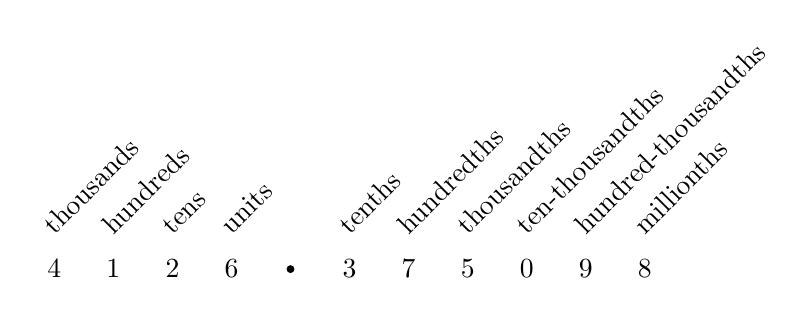
\begin{tikzpicture}
	\foreach \x in {0.75} {
		\draw (-4*\x,0) node[below]{4};
		\draw (-4*\x,0) node[above, anchor=south west, rotate=45]{thousands};
		\draw (-3*\x,0) node[below]{1};
		\draw (-3*\x,0) node[above, anchor=south west, rotate=45]{hundreds};
		\draw (-2*\x,0) node[below]{2};
		\draw (-2*\x,0) node[above, anchor=south west, rotate=45]{tens};
		\draw (-1*\x,0) node[below]{6};
		\draw (-1*\x,0) node[above, anchor=south west, rotate=45]{units};
		\fill (0,-0.25) circle[radius=0.05];
		\draw (1*\x,0) node[below]{3};
		\draw (1*\x,0) node[above, anchor=south west, rotate=45]{tenths};
		\draw (2*\x,0) node[below]{7};
		\draw (2*\x,0) node[above, anchor=south west, rotate=45]{hundredths};
		\draw (3*\x,0) node[below]{5};
		\draw (3*\x,0) node[above, anchor=south west, rotate=45]{thousandths};
		\draw (4*\x,0) node[below]{0};
		\draw (4*\x,0) node[above, anchor=south west, rotate=45]{ten-thousandths};
		\draw (5*\x,0) node[below]{9};
		\draw (5*\x,0) node[above, anchor=south west, rotate=45]{hundred-thousandths};
		\draw (6*\x,0) node[below]{8};
		\draw (6*\x,0) node[above, anchor=south west, rotate=45]{millionths};
	}
\end{tikzpicture}
\end{center}

To read the decimal 0.375, we can say ``zero point three seven five'', but this isn't very helpful. Instead, we read the number using place value and say ``three hundred seventy-five \textit{thousandths}''. Now, if someone were to say that number aloud, it sounds just like the fraction \[\frac{375}{1000}.\] In fact, this decimal number and this fraction represent exactly the same value. Of course, the fraction isn't in simplest form yet, but that's easy to fix: \[0.375 = \frac{375}{1000} = \frac{3}{8}\].

We have accomplished the goal of turning a terminating decimal into a fraction. The technique is simply to read the decimal aloud using its place value, and then write down the fraction we hear.

\subsubsection{Repeating decimals into fractions}

The ``read the number with its place value'' technique won't work for repeating decimals. (Why not?) Instead, we'll use some clever applications of the techniques we learned when solving equations.

Suppose we try to write the repeating decimal $0.\overline{4}$ as a fraction. Let's give this number a name so that we can do some algebraic manipulations. \[x = 0.\overline{4}\] Our goal will be to find an alternative way of writing $x$. To do that, we're going to make two clever moves.

The first clever move is to use MPOE: we will multiply both sides of this equation by 10. Multiplying $0.\overline{4}$ by 10 moves the decimal point one place to the right. But remember, the 4's repeat \textit{forever}, so there are \textit{still infinitely many} 4's to the right of the decimal point! We have: \[10x = 4.\overline{4}\]

The second clever move is to use an idea from when we were solving systems of equations: the elimination method. Watch what happens when we subtact the first equation we wrote from the second equation:

\[\begin{aligned}
	&&	10x &= 4.\overline{4}\\
- 	&& 	x 	&= 0.\overline{4}\\\hline
	&&	9x 	&= 4.0
\end{aligned}\]

Notice that the two numbers on the righthand side of our equations are exactly four units apart. In other words: the infinitely long tail of 4's disappears when we subtract! Now all we have to do is use DPOE to isolate $x$: \[9x = 4 \quad\implies\quad x = \frac{4}{9}\] If you have a calculator handy, you can perform this division and see that we have accomplished the goal of turning our repeating decimal into a fraction:\[0.\overline{4} = \frac{4}{9}\]

This process is sometimes called \textit{killing the tail}, since our goal is to subtract two different decimal forms that have the same repeating part, thereby eliminating the infintely long tail of digits.\footnote{An alternative technique, which we'll discuss in Algebra 2, involves turning the repeating decimal into an infinitely long sequence of ever-decreasing numbers, and then finding the sum of that sequence. Yes, we can -- in certain circumstances -- add up infinitely many numbers. This is just one of the amazing things that awaits you in Algebra 2!}

\begin{boxex}
Convert the repeating decimal $0.\overline{63}$ to its decimal representation.

\exsoln\ We'll kill the tail again, but note that we have two digits after the decimal which repeat. This will require a slight adjustment. We'll start as we did before, by assigning an algebraic name to our number:\[x = 0.6363\dotso\]
If we multiply both sides by 10, we'll have \[10x = 6.3636\dotso\] which is also a repeating decimal, but with a \textit{different} repeating tail. We could work with this, but it's a bit easier to multiply by 10 again (in other words, to multiply the original equation by 100): \[100x = 63.6363\dotso\] Now we have an equation in which the number on the righthand side has exactly the same tail as in the original equation. So, we subtract:
\[\begin{aligned}
	&&	100x	&= &63.\overline{63}\\
- 	&& 	x 		&= &0.\overline{63}\\\hline
	&&	99x 	&= &63.00
\end{aligned}\] We divide both sides by 99, and then simplify our fraction to lowest terms. In the end, we have: \[0.\overline{63} = \frac{63}{99} = \frac{7}{11}\]
\end{boxex}

The moral of the story is that we may have to adjust our method and choose the ``just right'' powers of 10. Consider how we might use kill the tail to turn $0.1\overline{6}$ back into $\frac{1}{6}$? (Note that the 6 repeats in the decimal form, but the 1 does not.)

Let's pause to reflect. In the first part of this section, we explained why every fraction can be written as either a terminating or repeating decimal. We can make this conversion using long division. Then we went on to show the reverse: that every terminating decimal can be written as a fraction (by reading it with its place value) and every repeating decimal can be written as a fraction (by killing the tail).

Armed with these tools, we might get the idea that \textit{every decimal} number can be turned into a fraction. Unfortunately (or fortunately, depending on how you look at it), this is not the case.

\subsection{Existence of irrational numbers}

The \glspl{irrational number} are all of the real numbers that are not rational numbers. In other words, those decimal numbers that cannot be expressed as either a terminating or repeating decimal.

Back in \cref{ch:numbers} we gave an example of such a number: \[0.10\,110\,1110\,11110\,111110\ldots\]
This number clearly has a pattern. We might explain it by saying: ``After the decimal point write one, then zero, the 2 ones, then zero, then 3 ones, then zero, and so on, always writing 1 more one than you did the last time.'' The problem is that is does not terminate (our pattern will continue forever), but it doesn't repeat either. The strings of 1's get longer and longer. There is never a set of always-repeating digits to group under a vinculum.

This single number is enough to prove that irrational numbers exist. Of course, there are lots of them. The famous number $\pi$ is irrational, and in some sense is even more diabolical.
\[\pi \approx 3. \, 1415926535 ~ 8979323846 ~ 2643383279 ~ 502884197 ~ 6939937510 ~ 5820974944 ~ 5923078164\ldots\]
This number doesn't even have a pattern that we can use to describe it (as far as we know). The digits go on infinitely, and come in a random sequence.

You may be wondering, ``How do we know $\pi$ is irrational?'' After all, it may be clear why the first number with the ones and zeros is irrational, but how to we know for sure that $\pi$ never terminates and never repeats?

Unfortunately, explaining the irrationality of $\pi$ requires a bit more mathematics that we can get into here. However, we have learned enough to prove that certain other numbers are irrational. More on that at the end of \cref{sec:radsquareroots}.

% % % % % % % % % % % % % % % % % % % % % % % % % % % % % % % % % % % % % % % % 
\section{Square roots}
\label{sec:radsquareroots}

We have already worked quite a bit with exponents, but every exponent so far has been an integer. Could we have a rational number as an exponent? If so, what would it mean?

\begin{boxexplore}[Half power]
Consider the expression \[9^{1/2},\] that is, ``nine to the power one-half''. What are some possible interpretations of this?

Use a calculator to explore what happens when we raise certain numbers to the one-half power (start with the natural numbers between 1 and 20). What patterns do you notice? What conjectures do you have about what's happening?
\end{boxexplore}

Suppose we let $x = 9^{1/2}$. We'd like to find an alternative way of expressing $x$ that uses only integer exponents. One approach is to multiply each side of this equation by itself. Then we'd have:
\[\begin{aligned}
x 			&= 9^{1/2}\\
x\cdot x 	&= 9^{1/2} \cdot 9^{1/2}
&&\quad\text{multiply each side by itself}\\
x\cdot x	&= 9^{(1/2)\,+\,(1/2)}
&&\quad\text{product rule for exponents}\\
x\cdot x	&= 9^{1}\\
x\cdot x	&= 9
\end{aligned}\]
So, $x$ is the number that when multiplied by itself gives $9$ as the result. That could be either $3$ or $\umin3$, since $3\cdot 3 = \umin3 \cdot \umin3 = 9$. Using some vocabulary that we already know: we say that $9^{1/2}$ is a \textit{square root} of $9$.

\begin{boxdef}[Square root]
A \gls{square root} of $a$ is a number $b$ such that $b \cdot b = a$.
\end{boxdef}

The reason this is called a ``square root'' has to do with the geometric interpretation of this operation. If we have a square of side length $\mathcal{S}$, then the area of the square is $\mathcal{S}^2$. Conversely, if we have a square with area $\mathcal{A}$, then the \textit{square root of $\mathcal{A}$} gives us the side length of the square. 

\begin{center}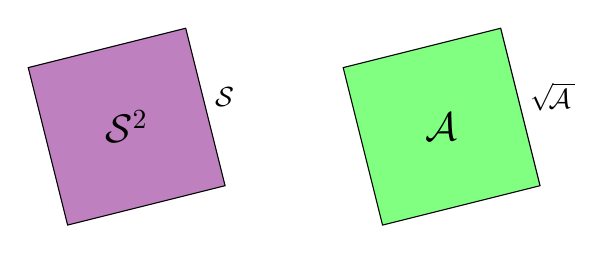
\begin{tikzpicture}[scale=0.5]
	\draw[fill=violet!50] (0,0) -- (4,1) -- (3,5) -- (-1,4) -- cycle;
	\draw (3.5,3.25) node[right]{$\mathcal{S}$};
	\draw (1.5, 2.5) node{\Large$\mathcal{S}^2$};
	\draw[fill=green!50] (8,0) -- (12,1) -- (11,5) -- (7,4) -- cycle;
	\draw (11.5,3.25) node[right]{$\sqrt{\!\mathcal{A}\,}$};
	\draw (9.5, 2.5) node{\Large$\mathcal{A}$};
\end{tikzpicture}\end{center}

Positive numbers have two square roots: one positive, one negative. Both 3 and $\umin3$ are square roots of 9, since $(3)(3) = 9$ and $(\umin3)(\umin3) = 9$. Zero is the only number that has exactly one square root: the square root of 0 is 0. Negative numbers cause some problems when it comes to square roots (stay tuned for more on that).

Most of the time, we'll be working with the positive square root of a number, called the \gls{principal square root} For example, the principal square root of 9 is 3 and the principal square root of 25 is 5.

The checkmark-ish symbol we use to denote the square root of $a$ is called the \gls{radical}: $\sqrt{a}$. This symbol means ``the principal square root of $a$''. So, $\sqrt{9} = 3$ and $\sqrt{25} = 5$. So, although $\umin3$ is a square root of 9, it is incorrect to write $\sqrt{9} = \umin3$ or $\sqrt{9} = \pm3$. This isn't quite rise to the level of \evilandwrong, but it's not right.\footnote{An algebra note from the future! When we simplify the expression $\sqrt{m^2}$, the result is $\abs{m}$, the absolute value of $m$. Do you see why? The value that comes out of the radical must be positive, because that notation gives the principal square root.}

When simplifying an expression or solving an equation, we won't always give both square roots.  A good guideline as we go along is to pay close attention and use the notation given in the problem. For example: \[\pm\sqrt{100} = \pm10 \qquad\text{and}\qquad -\sqrt{36} = \umin6\]
In these cases, the notation specifically indicates that we want both the positive and negative square root, or only the negative square root.

%%% Move to later, when solving equations?
%An Issue of Notation Now, squaring a number does something special. It gets rid of any negatives that may be attached to the number. So, when you square a number, you eliminate the sign. So, when you ``undo'' the square and take the square root, especially when solving an equation, you don't know if the original was positive or negative and you really get two solutions that actually work!
%
%Since you don't know which to give you give both. Of course when using square roots with the Pythagorean theorem, we ignore the negative root because distances aren't negative.
%
%So, if you choose to add the square root into a problem, you have to put the +/- in it. When you see it written in an expression, you are told which one you have. You need to remember this when you are simplifying a radical or solving an equation with a radical in it.

\subsection{Imaginary numbers}

Consider the expression $\sqrt{\umin16}$. This is a bit of a problem. We're meant to find the principal square root of $\umin16$, but the closest we can get is $4 \cdot \umin4 = \umin16$. It's true that $4$ and $\umin4$ have the same absolute value, but they're not the same number, which means we're not \textit{squaring} anything. So, there is no real number equal to $\sqrt{\umin16}$. Of course, $\umin16$ isn't special, the same argument applies to any negative number.

\begin{boxdef}[Square root of a negative number]
If $a < 0$, then there is no real number equal to $\sqrt{a}$.
\end{boxdef}

Note that this \textit{doesn't} mean that $\umin16$ doesn't have any square roots. It simply means that the square roots are not real numbers. The square roots of $\umin16$ are members of a set called the \textit{complex numbers} $\C$, but not members of the real numbers $\R$.

To build up the complex numbers, we introduce the so-called imaginary unit $\iu$ which has the property that $\iu^2 = −1$. Remember, the domain of Algebra 1 is the set real numbers. But, the domain of Algebra 2 and beyond is the set of complex numbers. So, if you're intrigued about imaginary numbers, just hang in there.

Our work in Algebra 1 will bring us mostly in contact with \textit{square roots}, but other roots are possible. For example a ``cube root'' of a number $a$ is a number $b$ such that $b\cdot b\cdot b = a$. We write $\sqrt[3]{a}$ to denote the cube root of $a$. Negative numbers under the cube root symbol are no problem: \[\sqrt[3]{\umin8} = \umin2 \qquad\text{since}\qquad \umin2\cdot\umin2\cdot\umin2 = \umin8\]


\subsection{(;,;) Irrationality of the square root of two}

We have shown that irrational numbers exist. Consider the mathematical argument below, which explains why the square root of 2 is irrational.

\textit{Step 1.~} Assume (for the moment) that $\sqrt{2}$ is, in fact, rational. In other words, that it can be written as the ratio of two integers. Then, we can write \[\sqrt{2} = \frac{a}{b}\] where $a$ and $b$ are relatively prime. That is to say, our fraction is in lowest terms.

\textit{Step 2.~} Square both sides of the equation above. \[2 = \frac{a^2}{b^2}\]

\textit{Step 3.~} Multiply both sides of this equation by $b^2$. \[2b^2 = a^2\] This means that $a^2$ is an even number. If $a^2$ is an even number, then $a$ must be an even number.

\textit{Step 4.~} If $a$ is an even number, then it is divisible by 2. In other words, there is an integer $m$ such that $a = 2m$.

\textit{Step 5.~} Substitute $2m$ for $a$ in the equation from Step 3, and simplify.\[\begin{aligned} 2b^2 &= (2m)^2 \\ 2b^2 &= 4m^2 \\ b^2 &= 2m^2 \end{aligned}\] This means that $b^2$ is an even number. If $b^2$ is an even number, then $b$ is an even number.

\textit{Step 6.~} If both $a$ and $b$ are even numbers, then the original fraction $\frac{a}{b}$ was not in lowest terms, which was our assumption! This contradiction shows that our original assumption cannot be true.

Thus, $\sqrt{2}$ cannot be written as a fraction. In other words, $\sqrt2$ is an irrational number.

\subsubsection{Thoughts to chew on}

Steps 3 and 5 both include assertions about numbers being even. How do we know when a number is even? Specifically, how do we know that $a^2$ and $b^2$ are even?

Steps 3 and 5 both go on to say something like ``if $a^2$ is even, then $a$ is even''. How do we know this is true? Under what circumstances will the square of a number be even or odd?

Step 6 argues that $\frac{a}{b}$ is not in lowest terms. How do we know this is true?

This is an example of \textit{proof by contradiction}. We assume that some statement is true, then show that this assumption leads to some kind of impossible situation. The impossibility means we have to reject the original assumption. What was our original assumption in this proof? What is the contradiction that results from that assumption?\footnote{Another famous proof by contradiction is Euclid's proof that there are infinitely many prime numbers. Have a look in \cref{app:primes}!}

% % % % % % % % % % % % % % % % % % % % % % % % % % % % % % % % % % % % % % % % 
\section{Simplified radical form}
\label{sec:radsimplifiedform}

%\begin{boxexplore}[TODO]
%TODO
%\end{boxexplore}
\addtodoitem{Startup exploration on simplified radical form?}

%When we take the square root of a perfect square we get an integer as the answer. It may come in handy to memorize the first 25 or so perfect squares, so that you can recognize them when they come up in a problem.

%\begin{center}
%\begin{tabular}{*{5}{C{0.15\textwidth}}}
%1^2 = 1	 &
%2^2 = 4	 &
%3^2 = 9	 &
%4^2 = 16 &
%5^2 = 25 \\
%6^2 = 36 &
%7^2 = 49 &
%8^2 = 64 &
%9^2 = 81 &
%10^2 = 100 \\
%11^2 = 121 &
%12^2 = 144 &
%13^2 = 169 &
%14^2 = 196 &
%15^2 = 225 \\
%16^2 = 256 &
%17^2 = 289 &
%18^2 = 324 &
%19^2 = 361 &
%20^2 = 400 \\
%21^2 = 441 &
%22^2 = 484 &
%23^2 = 529 &
%24^2 = 576 &
%25^2 = 625 \\
%\end{tabular}
%\end{center}

When we take the square root of a perfect square we get an integer as the answer. But, things are not so easy when taking the square root of a number that is not a perfect square. In fact, the square root of a non-square natural number will be an irrational number, like $\sqrt{2}$.

The \textit{exact value} of an irrational number can only be represented using some kind of symbol, like $\pi$ or $\sqrt2$. Writing out a decimal value -- no matter how many decimals you write down -- will always be an approximation. So, it's a good habit of mind to think ``should I be giving an exact answer to this problem, or is a decimal approximation good enough''. Very often, the context (or the directions) will make this choice clear.

To help us standardize the way we write radical expressions, we all agree to comply with \textit{simplified radical form}.

\begin{boxcrit}[Simplified radical form]
A radical expression is considered completely simplified if\ldots
\begin{enumerate}
\item Like radical terms have been combined.
\item The expression under the radical has no perfect square factors other than 1.
\item There are no fractions under the radical.
\item There are no radicals in the denominator of a fraction.
\end{enumerate}
\end{boxcrit}

Over the next few sections, we will discuss each of these criteria and the algebraic manipulations that we can use to make sure our expressions comply. The first criteria is quite straightforward, so let's get right to it.

\subsection{Like radical terms}

Criteria \#1 states that like radical terms must be combined. We combine radical terms as we do variable terms. For example, we are very familiar with the simplification \[x + x = 2x.\] We combine radical terms in exactly the same way: \[\sqrt5 + \sqrt5 = 2\cdot\sqrt5 = 2\sqrt5.\]
Note, in particular, that the sum here is not $\sqrt{10}$. Similarly, $3x + 4x = 7x$ and so with radicals, we have $3\sqrt{21} + 4\sqrt{21} = 7\sqrt{21}$. When we have a multiplication of a number times a radical, we can omit the multiplication symbol.

\addtodoitem{See Patty's alternative way of simplifying radicals.}

\begin{boxwarn}
When we say like radical terms ``can be combined'', don't go thinking you can add the numbers under the radical. To add the values like this is \evilandwrong.
\[ \sqrt{3} + \sqrt{3} \neq \sqrt{6}\]
Since a radical is like an exponent, this is the equivalent of saying $(a+b)^2=a^2+b^2$ which, by now, we know is not generally the case. You can't sprinkle that exponent across the sum!

While we're at it, don't get any ideas about splitting the radical-of-a-sum into the sum-of-radicals. This, too, is \evilandwrong.
\[\sqrt{2+14} \neq \sqrt{2} +\sqrt{14}\]
\end{boxwarn}


% % % % % % % % % % % % % % % % % % % % % % % % % % % % % % % % % % % % % % % % 
\subsection{Product properties of radicals}
%\label{sec:radproduct}

\begin{boxexplore}[Building blocks]
The number 1 is the \textit{additive building block} of the natural numbers. In other words: If we want to ``build'' any natural number using only addition, the only number we need is the number 1. Every natural number can be written as the sum of a bunch of 1's.

What are the \textit{multiplicative building blocks} of the natural numbers? Note that we have to say \textit{blocks} (plural) since the number 1 is not enough: multiplying together a bunch of 1's always gives us 1 as the product. What is the smallest collection of natural numbers that we need in order to build the rest using only multiplication?
\end{boxexplore}

The second criteria for simplified radical form states that the expression under the radical may have no perfect square factors other than 1. This may seem strangely worded. It clearly handles the idea that there should be no perfect squares under the radical, and that makes sense. Expressions like $\sqrt{4}$ and $\sqrt{25}$ can pretty obviously be simplified.

But, this criteria also catches expressions like $\sqrt{24}$ and $\sqrt{50}$ because those numbers, neither of which is a perfect square, each have a perfect square as a factor: 24 has 4 as a factor, and 50 has 25 as a factor.

How can we simplify an expression like $\sqrt{50}$ so that it has no perfect square factors under the radical? For help, we turn to:

\begin{boxdef}[Product rule of radicals]
For any $a \geq 0$ and $b \geq 0$, \[\sqrt{ab} = \sqrt{a} \cdot \sqrt{b}.\]

Note: In Algebra 1 we only use the square root version of this property, though in fact it applies to radicals of any degree: cube roots, fourth roots, and so on.
\end{boxdef}

This property looks an awful lot like the product rule for exponents, which makes sense since here we are undoing the power of a product rule, where the power is the exponent one-half!

\begin{boxex}
Express $\sqrt{50}$ in simplified radical form.

\exsoln\ We know $\sqrt{50}$ is not yet in simplified radical form because 50 is divisible by a perfect square, $50 = 25 \cdot 2$. We apply the multiplication property of radicals like so:
\[
\begin{aligned}
\sqrt{50} 	&= \sqrt{25 \cdot 2}
&& \quad \text{rewrite 50 to show its perfect square factor}\\
			&= \sqrt{25} \cdot \sqrt{2}
&& \quad \text{product rule of radicals}\\
			&= 5 \cdot \sqrt{2}
&& \quad \text{simplify the square root of a perfect square}
\end{aligned}
\]
So, $\sqrt{50} = 5\sqrt{2}$. These two expressions are equal, but only the second expression satisfies the criteria of simplified radical form.
\end{boxex}

\subsection{Different approaches to simplifying}

There are a number of ways to go about applying this property to simplify expressions. Use whatever approach makes the most sense to you! Here are some alternatives, though you might find a different approach that fits you better. In any case, it will probably be helpful to learn a variety of methods. Depending on the problem, some methods may be easier to use than others.

For example, let's examine different ways to get $\sqrt{108}$ into simplified radical form.

\subsubsection{Strategy 1: Largest square factor}

In this strategy, we find the largest perfect square factor and simplify it using the product rule for radicals. We might notice that $108 = 3 \times 36$: \[\sqrt{108} = \sqrt{36 \cdot 3} = \sqrt{36} \cdot \sqrt{3} = 6\sqrt{3}\]

\subsubsection{Strategy 2: One square at a time}

It might not be obvious what the largest perfect square is, so in this strategy we look for \textit{any} prefect square factor and work one square at a time. For instance, we might notice that 108 is divisible by 9 (how can we quickly spot divisibility by 9?). Then: \[\sqrt{108} = \sqrt{9 \cdot 12} = \sqrt{9} \cdot \sqrt{12} = 3 \cdot \sqrt{12} = 3 \cdot \sqrt{4 \cdot 3} = 3 \cdot \sqrt{4} \cdot \sqrt{3} = 3 \cdot 2 \cdot \sqrt{3} = 6\sqrt{3}\]

In this approach, we have to keep checking to see whether the number under the radical is ``square-free'' or not. After our first simplification, we have 12 under the radical. But 12 has 4 as a factor, so we have to do another simplification step.

This process might take a little longer, but it is sometimes easier to identify smaller perfect square factors and chip away at the problem, than it is to identify the largest perfect square factor and finish the problem in a single step.

\subsubsection{Strategy 3: Sniper method}

The idea here is to write the \textit{prime factorization} of the number under the radical, and then look for pairs of factors.\footnote{One way to break a number down into primes is using a factor tree. For a handy, if unusually-formatted, list of prime numbers, see \cref{app:primes}.} The factorization of $108 = 2 \cdot 2 \cdot 3 \cdot 3 \cdot 3$, so: \[\sqrt{108} = \sqrt{\underline{\color{blue}2 \cdot 2} \cdot \underline{\color{red}3 \cdot 3} \cdot 3} = \underline{\color{blue}2} \cdot \underline{\color{red}3} \cdot \sqrt{3} = 6\sqrt{3} \]

We've given this strategy the memorable (though perhaps gruesome) name \textit{the sniper method}. Think of the radical as a prison. There are snipers outside and any number that tries to escape needs to have a decoy. A single factor of 2 is stuck inside for life, but if the 2 has a partner (that is, if there's a $2 \cdot 2$ under the radical), then 2 can make a break for it!

But, only one of the partners survives the jailbreak. The snipers take out the decoy. In the example above, one 2 makes it out, and so does one 3. The final factor of 3 is partnerless, and left trapped inside its radical prison.

\begin{boxex}
	TO DO.
\end{boxex}

% % % % % % % % % % % % % % % % % % % % % % % % % % % % % % % % % % % % % % % % 
\subsection{Quotient properties of radicals}
\label{sec:radquotient}

Criteria \#3 and \#4 for simplified radical form are both pretty antiquated. They came about in the pre-calculator days when folks had to do a lot more calculation by hand and use large data tables to approximate radical values. Yet, these last two properties are still considered ``standard'' for simplified radical form.

\addtodoitem{Image of a sliderule?}

Rules were made to be broken, though, and there will be times when it's OK to break away from these criteria (\#4 especially). But we'll burn that bridge when we come to it. For now, all four criteria are in effect.

Both of these have to do with interactions between radicals and fractions. Criteria \#3 disallows fractions under the radical, and criteria \#4 forbids radicals in the denominator of a fraction.

To tackle Criteria \#3, for example when faced with expressions like \[\sqrt{\frac{4}{49}} \quad\text{or}\quad \sqrt{\frac{24}{25}}~,\]we turn to:

\begin{boxdef}[Quotient rule of radicals]
For any $a \geq 0$ and $b \geq 0$, \[\sqrt{\frac{a}{b}} = \dfrac{\sqrt{a}}{\sqrt{b}}.\]
\end{boxdef}

Again, this property applies to radicals of any degree (though for now we'll focus on square roots). And again, this property is just like the quotient rule for exponents, but with a rational exponent.

\begin{boxex}
Express $\sqrt{\frac{4}{49}}$ and $\sqrt{\frac{24}{25}}$ in simplified radical form.

\exsoln\ Here we have a fairly clear application of the rule:
\[\begin{aligned}
\sqrt{\frac{4}{49}}	&= \frac{\sqrt{4}}{\sqrt{49}}
&& \text{\quad quotient rule of radicals}\\[1ex]
&= \frac{2}{7}
&& \text{\quad simplify sqaure roots}\\
\end{aligned}
\]
In the second example, the numerator doesn't contain in a perfect square, so we must apply the product rule.
\[\begin{aligned}
\sqrt{\frac{24}{25}}	&= \frac{\sqrt{24}}{\sqrt{25}}
&& \text{\quad quotient rule of radicals}\\[1ex]
&= \frac{\sqrt{24}}{5}
&& \text{\quad simplify denominator}\\[1ex]
&= \frac{\sqrt{4\cdot6}}{5}
&& \text{\quad product rule in the numerator}\\[1ex]
&= \frac{\sqrt{4}\cdot\sqrt{6}}{5}\\[1ex]
&= \frac{2\sqrt{6}}{5}
\end{aligned}
\]
\end{boxex}

\subsection{Rationalizing the denominator}

When simplifying an expression using the division property, we may encounter something like the following: \[\sqrt{\frac{9}{2}} = \frac{\sqrt{9}}{\sqrt{2}} = \frac{3}{\sqrt{2}}\]
Back in the pre-calculator days, this led to criteria \#4, no radicals in the denominator of a fraction. After all, long division is bad enough to carry out by hand. Why not try to put yourself into a situation that makes division as easy and accurate as possible, and avoid dividing by a big ugly decimal?

When we have a radical in the denominator of a fraction we have an \textit{irrational denominator}. Our goal is to fix this by creating an equivalent fraction with a \textit{rational denominator}. The process of making this translation is called \gls{rationalizing the denominator}.

We will employ the trusty \textit{identity property of multiplication}. Remember, multiplying a number by a fancy 1 does not change the value of the number. The trick will be to choose the way our version of 1 looks. We are going to choose a fancy version of 1 that when multiplied by our irrational denominator gives us a rational number (in fact, an integer).

Study the following examples:

\begin{boxex}
Write $\dfrac{3}{\sqrt{2}}$ in simplified radical form.

\exsoln\ Note the clever use of multiplication by a fancy version of 1.
\[\begin{aligned}
\dfrac{3}{\sqrt{2}} &= \dfrac{3}{\sqrt{2}} \cdot 1
&&\quad\text{identity property of multiplication}\\
&= \dfrac{3}{\sqrt{2}} \cdot \dfrac{\sqrt{2}}{\sqrt{2}}
&&\quad\text{substitute a fancy version of 1}\\
&=~ \dfrac{3 \sqrt{2}}{\sqrt{2} \cdot \sqrt{2}}
&&\quad\text{multiply fractions}\\
&=~ \dfrac{3 \sqrt{2}}{2}
&&\quad\text{definition of square root (in the denominator)}\\
\end{aligned}
\]
\end{boxex}

Note that we chose as our fancy 1 \textit{exactly what we needed} to make the denominator of our fraction turn into an integer. This might seem like cheating, but it's a completely legal move, algebraically speaking.

Be sure to pay close attention. Sometimes we can use the division property in reverse to get rid of radicals in the denominator. We'll work the next example in two different ways to show the comparison.

\begin{boxex}
Write $\dfrac{\sqrt{84}}{\sqrt{6}}$ in simplified radical form.

\exsoln\ First, we'll rationalize the denominator using a fancy version of 1.
\[\begin{aligned}
\dfrac{\sqrt{84}}{\sqrt{6}} &= \dfrac{\sqrt{84}}{\sqrt{6}} \cdot 1
&&\quad\text{identity property of multiplication}
\\[1ex]
&= \dfrac{\sqrt{84}}{\sqrt{6}} \cdot \dfrac{\sqrt{6}}{\sqrt{6}}
&&\quad\text{substitute a fancy version of 1}
\\[1ex]
&=~ \dfrac{\sqrt{84} \cdot \sqrt{6}}{\sqrt{6} \cdot \sqrt{6}}
&&\quad\text{multiply fractions}
\\[1ex]
&=~ \dfrac{\sqrt{{\color{blue}84} \cdot {\color{red}6}}}{6}
&&\quad\text{product rule for radicals}
\\[1ex]
&=~ \dfrac{\sqrt{{\color{blue}2 \cdot 2 \cdot 3 \cdot 7} \cdot {\color{red}3 \cdot 2}}}{6}
&&\quad\text{simplify numerator using the sniper method}
\\[1ex]
&=~ \dfrac{2 \cdot 3 \sqrt{2 \cdot 7}}{6}
&&\quad\text{}
\\[1ex]
&=~ \dfrac{6 \sqrt{14}}{6}
&&\quad\text{}
\\[1ex]
&=~ \sqrt{14}
&&\quad\text{}\\
\end{aligned}
\]

Now, an alternative approach: We'll use the division property of radicals in reverse first, and then simplify the fraction under the radical.
\[\begin{aligned}
\dfrac{\sqrt{84}}{\sqrt{6}} &= \sqrt{\dfrac{84}{6}}
&&\quad\text{division property of radicals}
\\[1ex]
&=~ \sqrt{\dfrac{14}{1}}
&&\quad\text{simplify the fraction}
\\[1ex]
&=~ \sqrt{14}
&&\quad\text{Voil\`a.}
\end{aligned}
\]
\end{boxex}

The second approach is much easier in this case. It pays to work smart and do a bit of planning before charging ahead with an algorithm blindly. It may not always be this easy, though. Under what circumstances will we be able to use the kind of shortcut?

\begin{boxwarn}
Answers with fractions must be simplified, but folks sometimes get overly aggressive with the simplification. Consider the following: \[\frac{2}{\sqrt{6}} = \frac{2}{\sqrt{6}}\cdot\frac{\sqrt{6}}{\sqrt{6}} = \frac{2\sqrt{6}}{\sqrt{6}\cdot\sqrt{6}} = \frac{2\sqrt{6}}{6}\]
At this point, we can do one more simplification: \[\frac{2\sqrt{6}}{6} = \frac{\sqrt{6}}{3} \qquad \text{Yes!}\]
But we might be tempted to try and simplify even more: \[\frac{\sqrt{6}}{3} = \frac{\sqrt{2}}{1} \qquad \text{No!}\]
It's tempting, but we can't simplify using things \textit{under} the radical and things \textit{outside} the radical. That 6 under the radical cannot cancel with the 3 outside! To attempt such a simplification is \evilandwrong.
\end{boxwarn}

\begin{boxex}
Determine the value of $x$ given the equation: $2x^2+4x-3=40$.

\exsoln\ We'll use everything that we learned in \cref{ch:quadeq}! Our first step is to ensure that the first term is a perfect square, so we multiply through by 2.
\[4x^2 + 8x - 6 = 80\]
This also gives us an even linear coefficient, so it looks like we're ready for the quadrangle method.
\begin{center}
\quadrangle{2x}{2}{4x^2}{4x}{\color{red}4}
\end{center}
The quadrangle method predicts 4 as the constant term, but our equation has $-6$. APOE to the rescue:
\begin{align*}
4x^2 + 8x - 6 &= 80
\\
4x^2 + 8x + 4 &= 90
&&\text{APOE: add 10 to both sides}
\\
(2x+2)^2 &= 90
&&\text{based on the quadrangle diagram}
\\
2x+2 &= \pm\sqrt{90}
&&\text{square root of both sides}
\\
2x &= -2 \pm\sqrt{90}
&&\text{SPOE}
\\[1ex]
x &= \frac{-2 \pm\sqrt{90}}{2}
&&\text{DPOE}
\end{align*}
Almost there! Remember, we need to simplify our radicals! We can use the sniper method in this case:
\[\sqrt{90} = \sqrt{3\cdot3\cdot2\cdot5} = 3\sqrt{2\cdot5} = 3\sqrt{10}.\]
And so in the end, we have
\[\solset{\frac{-2 \pm 3\sqrt{10}}{2}}\]
We'll admit that these answers ain't pretty (note that there are two answers there!), but they are the values that satisfy our original quadratic equation.
\end{boxex}

% % % % % % % % % % % % % % % % % % % % % % % % % % % % % % % % % % % % % % % % 
\section{Coordinate geometry}
\label{sec:coordgeometry}

\begin{boxexplore}[Squarea]
As we saw in \cref{sec:radsquareroots}, a square with area $\mathcal{A}$ has side length $\sqrt{\!\mathcal{A}\,}$. Consider the figures below.

\begin{center}
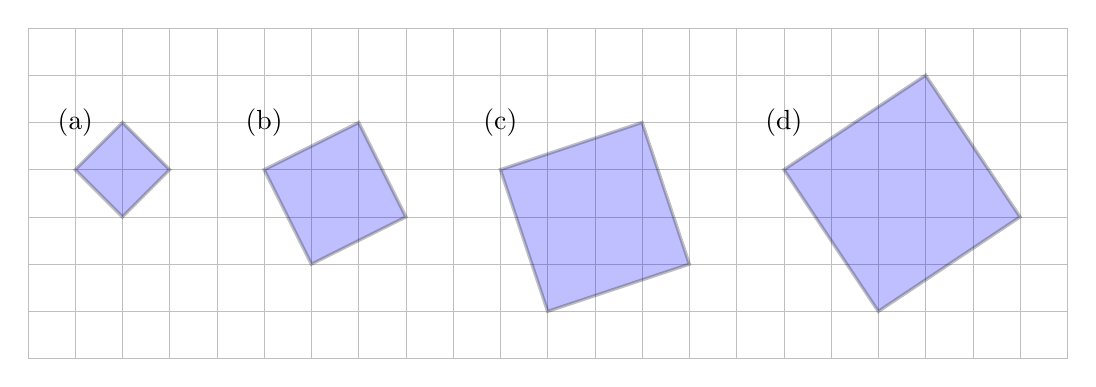
\begin{tikzpicture}[scale=0.6]
	\draw[black!25, very thin] (0,-1) grid (22,6);
	\draw(1,4) node{(a)};
	\draw[very thick, fill=blue, nearly transparent]
		(1,3) -- (2,2) -- (3,3) -- (2,4) -- cycle;
	\draw(5,4) node{(b)};
	\draw[very thick, fill=blue, nearly transparent]
		(5,3) -- (6,1) -- (8,2) -- (7,4) -- cycle;
	\draw(10,4) node{(c)};
	\draw[very thick, fill=blue, nearly transparent]
		(10,3) -- (11,0) -- (14,1) -- (13,4) -- cycle;
	\draw(16,4) node{(d)};
	\draw[very thick, fill=blue, nearly transparent]
		(16,3) -- (18,0) -- (21,2) -- (19,5) -- cycle;
\end{tikzpicture}
\end{center}

What is the area of each square? What is the side length of each square? Can you draw a square with side length $\sqrt{8}$? What about $\sqrt{13}$?

By the way, how do we know that each of these figures is, in fact, a square? (Hint: Think back to the slopes of parallel and perpendicular lines. What argument can we make for why the diagonal segments must be the same length in each figure?)
\end{boxexplore}

As an application of radicals and radical expressions, which are closely connected to the side lengths of squares, it's natural to discuss concepts from geometry. We'll begin with one of the most famous and important statements in mathematics.

\subsection{{P}ythagorean theorem}

It's a good bet that have seen the Pythagorean Theorem before, and that you will see it in every high school mathematics class you take, and many of the mathematics classed you take in college. In fact, the Pythagorean theorem is a foundational piece of an entire branch of mathematics based on the properties of triangles called \textit{trigonometry}.\footnote{Trigonometry begins with the study of triangles. \textit{Trigon} is another way of sayinga \textit{triangle} -- in fact it might be a better way of naming that shape! Most of the other polygons we know (pentagons, hexagons, octagons) have that \textit{-gon} suffix, and the prefix \textit{tri-} means ``three'' (as in tricycle).}

\begin{boxdef}[{P}ythagorean theorem]
The sum of the squares of the lengths of the \glspl{leg} of a right triangle is equal to the square of the length of the \gls{hypotenuse}.

In other words, if $a$ and $b$ represent the lengths of the legs (the perpendicular sides) of a right triangle, and $c$ represents the length of the hypotenuse (the longest side, opposite the right angle), then \[a^2 + b^2 = c^2.\]
\end{boxdef}

The theorem is named after Greek philosopher and mathematician Pythagoras of Samos, who lived around 570--495 BCE.\footnote{\addtodoitem{Need a good Pythagoras footnote.}} However, there is substantial evidence that the theorem was known to many different cultures from many different time periods. There is evidence, for instance, that the ancient Babylonians knew about Pythagorean triples (see the next section) more than 1000 years BCE.

Let's jump in with a famous right triangle: one with legs of length 3 and 4, and with hypotenuse of length 5. If we draw squares on the sides of the triangle, we can see that the sums of the areas of the two smaller squares (9+16) is exactly equal to the area of the largest square (25).
\begin{center}
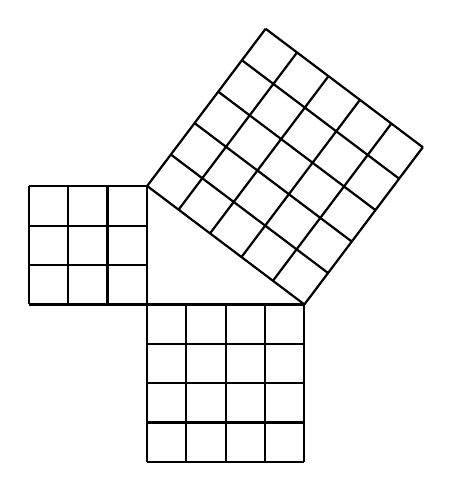
\begin{tikzpicture}[xscale=0.5,yscale=0.5]
	%% grid setup
	%\draw[very thin,color=gray!25] (0,0) grid (12,13);
	\draw[thick] (1,5) grid (4,8);
	\draw[thick] (4,1) grid (8,5);
	\draw[thick,rotate around={53:(8,5)}] (8,5) grid (13,10);
\end{tikzpicture}
\end{center}

This relationship holds true for all right triangles as does its \textit{converse}. The converse of the theorem states that if we have three numbers that satisfy the Pythagorean theorem, then we know that they must form the sides of a right triangle.

You might be asking yourself, ``How do we know that the theorem is true for \textit{every right triangle ever}?'' Those who are curious might enjoy exploring this question at the end of this section.

\subsection{{P}ythagorean triples}

\begin{boxdef}[{P}ythagorean triple]
A \textit{Pythagorean triple} is a set of three positive integers satisfying the Pythagorean theorem.
\end{boxdef}

There are infinitely many Pythagorean triples, and it is quite handy to know a few by heart. (This is because they are used quite a bit in problems, and those delightful standardized tests we all know and love.) Here are a few common Pythagorean triples:
\[
(3, 4, 5) \qquad\qquad
(5, 12, 13) \qquad\qquad
(7, 24, 25) \qquad\qquad
(9, 40, 41) \qquad\qquad
(8, 15, 17)
\]
The benefit of memorizing a few of these is that, if you see that a right triangle that has leg lengths of 7 and 24, you know that the hypotenuse has length 25 without having to do any calculations.

The triples above are called \inlinedef{primitive Pythagorean triples} because the three values are relatively prime. You can generate new Pythagorean triples by scaling up a triple that you know. For example $(6, 8, 10)$ is a triple formed by scaling up the $(3, 4, 5)$ triple by a factor of 2.

\subsubsection{Find-the-missing-side problems}

The classic application of the Pythagorean theorem is to find a missing side length, either a leg or a hypotenuse, and you may have solved problems like this before. Now that we have some algebra skills, however, our answers should be given in simplified radical form! No more decimal approximations (unless the directions state otherwise)!

\begin{boxex}
Find the length of the digaonal of a 4-by-8 rectangle.

\exsoln\ This problem might not, at first, seem to have anything to do with the Pythagorean theorem. The theorem, after all, is about right triangles, and this question is about a rectangle! Drawing a picture helps to reveal the connection:

\begin{center}\begin{tikzpicture}[scale=0.5]
	\draw[dashed] (0,0) -- (8,4);
	\draw (0,0) rectangle (8,4);
	\draw (4,0) node[below]{8};
	\draw (8,2) node[right]{4};
	\draw (4, 2) node[above]{$d$};
\end{tikzpicture}\end{center}

If we let $d$ represent the length of the diagonal, then we can see that it is the hypotenuse of a right triangle with legs of length 4 and 8. So:
\begin{align*}
d^2	&= 4^2 + 8^2
&&\quad\text{Pythagorean theorem}\\
d^2&= 16 + 64\\
d^2&= 80\\
d 	&= \sqrt{80}
&&\quad\text{square root of both sides}\\
d 	&= \sqrt{2 \cdot 2 \cdot 2 \cdot 2 \cdot 5}
&&\quad\text{simplify using the sniper method}\\
d 	&= 2 \cdot 2 \cdot \sqrt{5}\\
d 	&= 4\sqrt{5}
\end{align*}
So, a 4-by-8 rectangle has a diagonal which is $4\sqrt5$ units long.
\end{boxex}

To get a feel for whether this answer is reasonable, we could find a decimal approximation using a calculator (it's about 9 units long, which seems OK), or we could reason as follows. We know that $\sqrt{4} = 2$, and so $\sqrt{5}$ must be a bit more than 2. So, $4\sqrt{5}$ must be a bit more than 8. This seems reasonable.

On the other hand, if we had gotten $4\sqrt{8}$ we might reason that $\sqrt{9} = 3$ and so $4\sqrt{8}$ must be a bit less than $4\sqrt{9} = 4\cdot3 = 12$. This is too long for the diagonal of a 4-by-8 rectangle, since the two sides together are only 12 units long in total!

\subsection{Distance formula}

\begin{boxexplore}[Grid distance]
Find the length of the line segment connecting the points $(1,2)$ and $(6,7)$.
\end{boxexplore}

One important application of the Pythagorean theorem is called the \gls{distance formula}. It is a formula that we can use to calculate the distance between two points on a coordinate grid. In the startup exploration, we have the segment pictured below:

\begin{center}
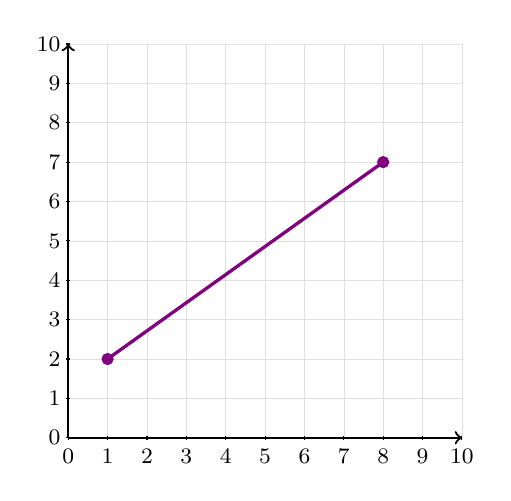
\begin{tikzpicture}[xscale=0.5,yscale=0.5]
	%% grid setup
	\draw[very thin, color=gray!25] (0,0) grid (10,10);
	\draw[->,thick] (0,0) -- (10,0); % node[right] {$x$};
	\draw[->,thick] (0,0) -- (0,10); % node[above] {$y$};
	\foreach \x in {0,...,10} \draw (\x,0.05) -- (\x,-0.05) node[below] {\footnotesize\x};
	\foreach \y in {0,...,10} \draw (-0.05,\y) -- (0.05,\y) node[left] {\footnotesize\y};
	\draw[very thick,violet] (1,2) -- (8,7); % node[right] {$x$};
	\draw[violet] plot[only marks,mark=*,mark size=4] coordinates{(1,2)(8,7)};
\end{tikzpicture}
\end{center}

If we think of the line segment into the hypotenuse of a right triangle, then we can use the Pythagorean theorem! The legs are the vertical and horizontal distances between the points, as in a slope triangle.

Draw the triangle, find the horizontal and vertical distances, then apply the Pythagorean theorem.

\begin{center}
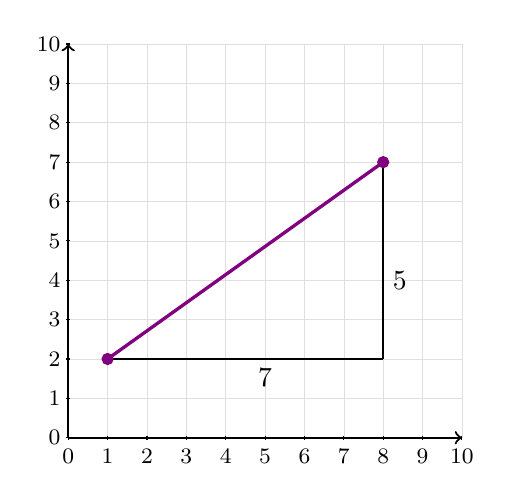
\begin{tikzpicture}[xscale=0.5,yscale=0.5]
	%% grid setup
	\draw[very thin, color=gray!25] (0,0) grid (10,10);
	\draw[->,thick] (0,0) -- (10,0); % node[right] {$x$};
	\draw[->,thick] (0,0) -- (0,10); % node[above] {$y$};
	\foreach \x in {0,...,10} \draw (\x,0.05) -- (\x,-0.05) node[below] {\footnotesize\x};
	\foreach \y in {0,...,10} \draw (-0.05,\y) -- (0.05,\y) node[left] {\footnotesize\y};
	\draw[very thick,violet] (1,2) -- (8,7); % node[right] {$x$};
	\draw[thick] (1,2) -- (8,2);
	\draw (5,2) node[below] {7};
	\draw[thick] (8,2) -- (8,7);
	\draw (8,4) node[right] {5};
	\draw[violet] plot[only marks,mark=*,mark size=4] coordinates{(1,2)(8,7)};
\end{tikzpicture}
\end{center}

The horizontal distance is 7 units, and the vertical distance is 5 units. Those are the legs of the right triangle. Then, we use the theorem to find the length of the hypotenuse: \[\begin{aligned} a^2 + b^2 &= c^2 \\ 5^2 + 7^2 &= c^2 \\ 25 + 49 &= c^2 \\ 74 &= c^2 \\ \sqrt{74} &= c\end{aligned}\]

Since the process is the same every time, we can generalize to find the distance between any two points $(x_1, y_1)$ and $(x_2, y_2)$ in the plane.

\begin{center}
\begin{tikzpicture}[xscale=0.5,yscale=0.5]
	%% grid setup
%	\draw[very thin, color=gray!25] (0,0) grid (10,10);
	\draw[->,thick] (0,0) -- (10,0); % node[right] {$x$};
	\draw[->,thick] (0,0) -- (0,10); % node[above] {$y$};
%	\foreach \x in {0,...,10} \draw (\x,0.05) -- (\x,-0.05) node[below] {\footnotesize\x};
%	\foreach \y in {0,...,10} \draw (-0.05,\y) -- (0.05,\y) node[left] {\footnotesize\y};
	%% line segment
	\draw[very thick,blue] (2,3) -- (8,7); % node[right] {$x$};
	%% horizontal labels
	\draw[dotted] (2,3) -- (2,0);
	\draw (2,0.1) -- (2,-0.1) node[below]{$x_1$};
	\draw[dotted] (8,7) -- (8,0);
	\draw (8,0.1) -- (8,-0.1) node[below]{$x_2$};
	%% vertical labels
	\draw[dotted] (2,3) -- (0,3);
	\draw (0.1,3) -- (-0.1,3) node[left]{$y_1$};
	\draw[dotted] (8,7) -- (0,7);
	\draw (0.1,7) -- (-0.1,7) node[left]{$y_2$};

%	\draw (1,2) node[below]{$(x_1, y_1)$};
%	\draw[thick] (1,2) -- (8,2);
%	\draw (5,2) node[below] {$x_2 - x_1$};
%	\draw[thick] (8,2) -- (8,7);
%	\draw (8,4) node[right] {$y_2 - y_1$};
	\draw[blue] plot[only marks,mark=*,mark size=4] coordinates{(2,3)(8,7)};
\end{tikzpicture}
\end{center}

\begin{boxdef}[Distance formula]
Given two points in the plane $(x_1, y_1)$ and $(x_2, y_2)$, the length $d$ of the line segment connecting the points is given by the formula:
\[d = \sqrt{ (x_2 - x_1)^2 + (y_2 - y_1)^2 }.\]
\end{boxdef}

This might look like a bunch of alphabet soup, much harder to remember than the Pythagorean theorem. But remember: this \textit{is} the Pythagorem theorem! If you forget the formula, don't panic! Just remember that the line segment between the two points is the hypotenuse of a right triangle.

\begin{boxex}
Find the distance between the points $(5, 12)$ and $(-4, -2)$.

\exsoln\ We will use the distance formula, but note that we have both subtraction and negative numbers. Watch those minus signs!
\[\begin{aligned}
d &= \sqrt{ (5 - \umin4)^2 + (12 - \umin2)^2 } \\
&= \sqrt{ 9^2 + 14^2 } \\
&=\sqrt{ 81 + 196 } \\
&=\sqrt{ 277 }
\end{aligned}\]
Since 277 is prime, we know our answer complies with simplified radical form, so we're all done. The distance betnwee the two points is $\sqrt{277}$ units.
\end{boxex}

\subsection{Midpoint formula}

When working with the distance formula, there is a related formula for finding the coordinates of \textit{midpoint} of a given line segment. Suppose we wanted to find the midpoint of the line segment connecting $(2,8)$ and $(8,4)$.
\begin{center}
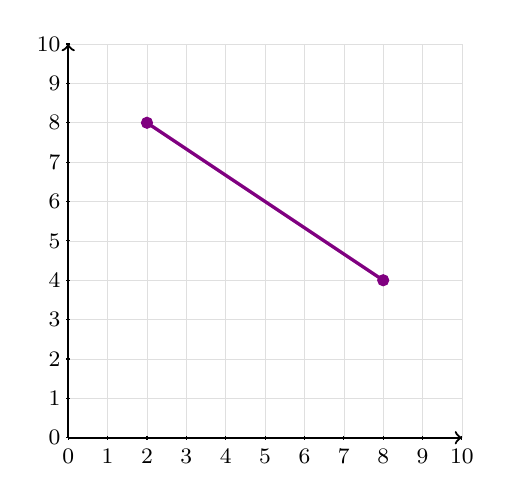
\begin{tikzpicture}[xscale=0.5,yscale=0.5]
	%% grid setup
	\draw[very thin, color=gray!25] (0,0) grid (10,10);
	\draw[->,thick] (0,0) -- (10,0); % node[right] {$x$};
	\draw[->,thick] (0,0) -- (0,10); % node[above] {$y$};
	\foreach \x in {0,...,10} \draw (\x,0.05) -- (\x,-0.05) node[below] {\footnotesize\x};
	\foreach \y in {0,...,10} \draw (-0.05,\y) -- (0.05,\y) node[left] {\footnotesize\y};
	\draw[very thick,violet] (2,8) -- (8,4); % node[right] {$x$};
	\draw[violet] plot[only marks,mark=*,mark size=4] coordinates{(2,8)(8,4)};
\end{tikzpicture}
\end{center}
Well, it sure looks like the midpoint of this segment is the point $(5,6)$\ldots\ but can we be sure?

One way to explain this is by drawing in the right triangle, and then chopping that triangle into four congruent sub-triangles. (Remember our work with the Sierpi\'{n}ski triangle ages ago?)
\begin{center}
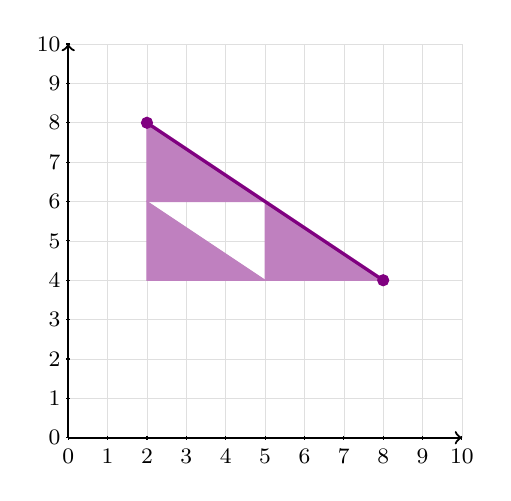
\begin{tikzpicture}[xscale=0.5,yscale=0.5]
	%% grid setup
	\draw[very thin, color=gray!25] (0,0) grid (10,10);
	\draw[->,thick] (0,0) -- (10,0); % node[right] {$x$};
	\draw[->,thick] (0,0) -- (0,10); % node[above] {$y$};
	\foreach \x in {0,...,10} \draw (\x,0.05) -- (\x,-0.05) node[below] {\footnotesize\x};
	\foreach \y in {0,...,10} \draw (-0.05,\y) -- (0.05,\y) node[left] {\footnotesize\y};
	\draw[violet!50, fill=violet!50] (2,8)--(2,6)--(5,6)--cycle;
	\draw[violet!50, fill=violet!50] (2,6)--(2,4)--(5,4)--cycle;
	\draw[violet!50, fill=violet!50] (5,6)--(5,4)--(8,4)--cycle;
	\draw[very thick,violet] (2,8) -- (8,4); % node[right] {$x$};
	\draw[violet] plot[only marks,mark=*,mark size=4] coordinates{(2,8)(8,4)};
\end{tikzpicture}
\end{center}
This diagram suggests that the $x$-coordinate of the midpoint of the hypotenuse is exactly halfway between the $x$-coordinates of the legs. The same goes for the $y$-coordinate. So, to find the coordinates of the midpoint, all we have to do is average the coordinates of the endpoints! Once again, you don't have to memorize this formula if you remember where it comes from!


\begin{boxdef}[Midpoint formula]
Given a line segment with endpoints $(x_1, y_1)$ and $(x_2, y_2)$, the coordinates of the midpoint of the segment are \[\left( \frac{x_1+x_2}{2} ~,~ \frac{y_1+y_2}{2} \right)\]
\end{boxdef}

\begin{boxex}
Find the midpoint of the segment connecting the points $(-13,8)$ and $(6, -2)$.

\inlineex{Solution:} Let's calculate the midpont first, and then check our answer by drawing a picture. The formula is pretty straightforward. The midpoint should be located at: \[\left( \frac{-13+6}{2} ~,~ \frac{8+\umin2}{2} \right) = \left( \frac{-7}{2} ~,~ \frac{6}{2} \right) = (-3.5, 3) \]
Here's a graph to check that our answer is reasonable:
\begin{center}
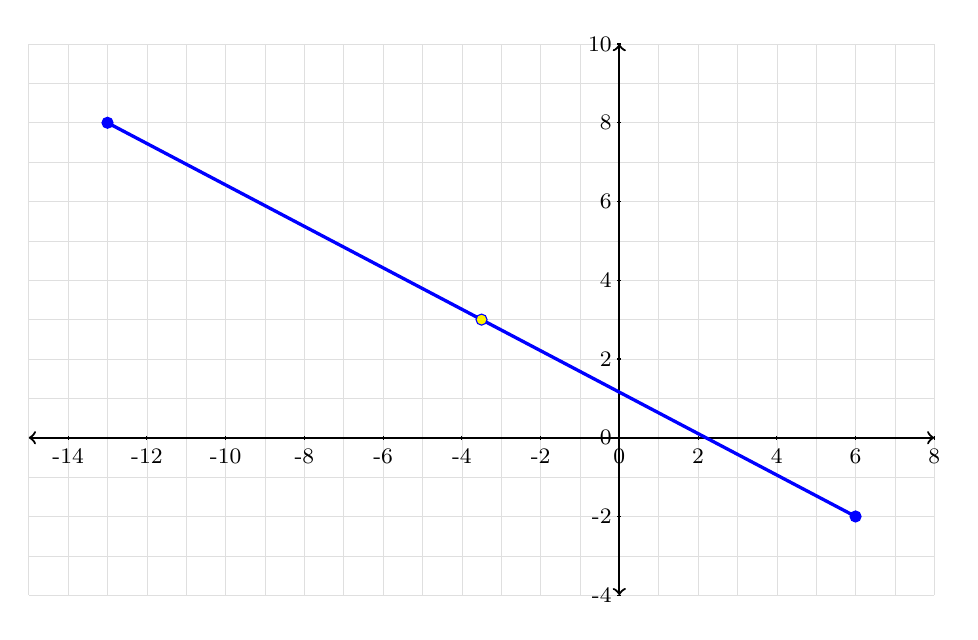
\begin{tikzpicture}[scale=0.5]
	%% grid setup
	\draw[very thin, color=gray!25] (-15,-4) grid (8, 10);
	\draw[<->,thick] (-15,0) -- (8,0);
	\draw[<->,thick] (0,-4) -- (0,10);
	\foreach \x in {-14,-12,...,8} \draw (\x,0.05) -- (\x,-0.05) node[below] {\footnotesize\x};
	\foreach \y in {-4,-2,...,10} \draw (-0.05,\y) -- (0.05,\y) node[left] {\footnotesize\y};
	%% line segment
	\draw[very thick,blue] (-13,8)--(6,-2);
	\draw[blue] plot[only marks,mark=*,mark size=4] coordinates{(-13,8)(6,-2)};
	\draw[blue, fill=yellow] plot[only marks,mark=*,mark size=4] coordinates{(-3.5,3)};
\end{tikzpicture}
\end{center}
\end{boxex}

\subsection{(;,;) Proof of the {P}ythagorean theorem}
\label{sec:pythagproof}

Imagine a pizza box and four identical slices of pizza\ldots\ where the pizza slices are right triangles. (Not typical for pizza slices, we know, but go with it.)

\begin{center}
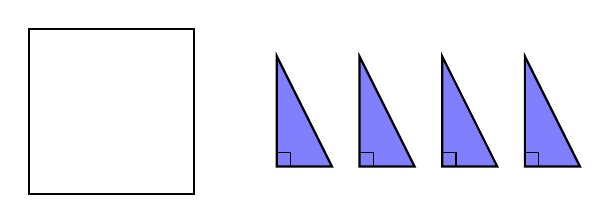
\begin{tikzpicture}[scale=0.35]
	\draw[thick] (0,0) rectangle (6,6);
	\foreach \x in {9,12,15,18} {
		\draw[thick, fill=blue!50] (\x,1) -- (\x+2,1) -- (\x,5) -- cycle;
		\draw (\x,1) rectangle (\x+0.5, 1.5);
	}
\end{tikzpicture}
\end{center}

Consider two different arrangements of the same four pizza slices inside the same pizza box. The slices are arranged to that they fit inside without overlapping, and they lay flat on the bottom of the box.

\begin{center}
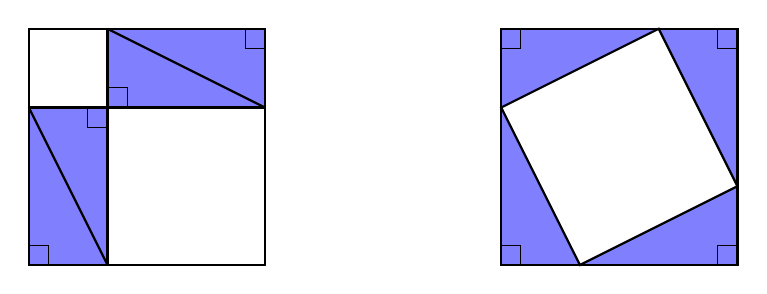
\begin{tikzpicture}[scale=0.5]
	%% Box 1
	\draw[thick] (0,0) rectangle (6,6);
	\draw[thick,fill=blue!50] (0,0) rectangle (2,4);
	\draw[thick,fill=blue!50] (2,4) rectangle (6,6);
	\draw (0,0) rectangle (0.5, 0.5);
	\draw (2,4) rectangle (1.5, 3.5);
	\draw (2,4) rectangle (2.5, 4.5);
	\draw (6,6) rectangle (5.5, 5.5);
	\draw[thick] (0,4) -- (2,0);
	\draw[thick] (2,6) -- (6,4);
	%% Box 2
	\begin{scope}[xshift=12cm]
	\draw[thick,fill=blue!50] (0,0) rectangle (6,6);
	\draw (0,0) rectangle (0.5, 0.5);
	\draw (0,6) rectangle (0.5, 5.5);
	\draw (6,0) rectangle (5.5, 0.5);
	\draw (6,6) rectangle (5.5, 5.5);
	\draw[thick,fill=white] (0,4) -- (2,0) -- (6,2) -- (4,6) -- cycle;
	\end{scope}
\end{tikzpicture}
\end{center}

\textit{Step 1:~} Consider the image on the left: Write an expression for the area of the box that is left \textit{uncovered}. You may find it helpful to label the sides of the triangles, or the sides of the box (or both).

You may be tempted to say that the uncovered regions are squares. How do we know -- for sure -- that these two regions are actually \textit{squares}, as opposed to some other quadrilateral?

\textit{Step 2:~} Consider the image on the right: Write an expression for the area of the box that is left \textit{uncovered}. Use the same labels you assigned when studying the other picture.

Again, you may be tempted to say that the uncovered region is a square. How do we know that it is a square (and not, say, a rhombus)?

\textit{Step 3:~} The area that is uncovered by the pizza slices is the same. (How do we know this?) What does this tell us about the two expressions for the uncovered area?

\subsubsection{Alternative approach}

In fact, we can explain the theorem using only the right-hand diagram. Let $a$ and $b$ be the lengths of the legs of one of the triangles, and let $c$ be the length of the hypotenuse.

\begin{center}
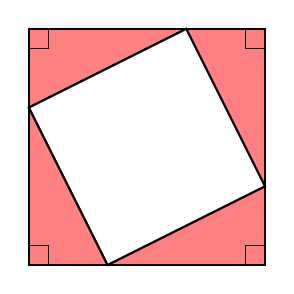
\begin{tikzpicture}[scale=0.5]
	%% Box 2
	\draw[thick,fill=red!50] (0,0) rectangle (6,6);
	\draw (0,0) rectangle (0.5, 0.5);
	\draw (0,6) rectangle (0.5, 5.5);
	\draw (6,0) rectangle (5.5, 0.5);
	\draw (6,6) rectangle (5.5, 5.5);
	\draw[thick,fill=white] (0,4) -- (2,0) -- (6,2) -- (4,6) -- cycle;
\end{tikzpicture}
\end{center}

\textit{Step 1:~} Express the sides of the largest square (the pizza box itself) in terms of $a$ and $b$.

\textit{Step 2:~} Express the area of the largest square in terms of $a$ and $b$. (Hint: You'll need the sum to a power rule.)

\textit{Step 3:~} The area of the largest square can also be expressed at the sum of the areas of the four triangles plus the area of the tiled square. Express the area of the largest square in this way (in terms of $a$, $b$, and $c$).

\textit{Step 4:~} We now have two ways of expressing the area of the largest square. What happens when set them equal to each other?

\subsubsection{Generalizing}

All the figures in this discussion have been drawn using a particular square and a particular triangle. Explain why these arguments are proof that the Pythagorean theorem is true for any right triangle, not just the specific triangle that is pictured in these diagrams.


% % % % % % % % % % % % % % % % % % % % % % % % % % % % % % % % % % % % % % % % 
\chaptersummary

Our algebra toolbox grows ever larger! We can now handle the simplification of numerical expressions that include square roots. This, combined with our work from the previous chapter, means that we can handle even the most ``impolite'' of quadratic equations. Plus, along the way we have discovered some fundamental results from geometry.

These skills are valuable, without a doubt, but we haven't looked closely at quadratic functions in detail. These are the focus of the next chapter. Onward!
